\begin{frame}{Applications}
  \begin{table}
    \scriptsize
    \centering
    \begin{tabular}{c c c c}
      \toprule
      Application & Knobs & Accuracy & Dataset \\
      \midrule
      \specialcell{Augmented\\Reality}
                  & \specialcell{resolution \\ frame rate \\ quantization }
                  & \specialcell{F1 score\\\cite{Rijsbergen:1979:IR:539927}}
                  & \specialcell{iPhone video clips\\training: office (24s)\\testing: home (246s)} \\
      
      \midrule
      \specialcell{Pedestrian\\Detection}
                  & \specialcell{resolution \\ frame rate \\ quantization }
                  & F1 score
                          & \specialcell{MOT16~\cite{milan2016mot16}\\training: MOT16-04\\testing: MOT16-03} \\
      \midrule
      \specialcell{Log Analysis\\(Top-K, K=50)}
                  & \specialcell{head (N) \\ threshold (T) }
                  & \specialcell{Kendall's $\tau$\\\cite{abdi2007kendall}}
                  & \specialcell{\href{https://www.sec.gov}{SEC.gov} logs~\cite{edgarlog} \\ training: 4 days \\
      testing: 16 days} \\
      \bottomrule
    \end{tabular}
  \end{table}

  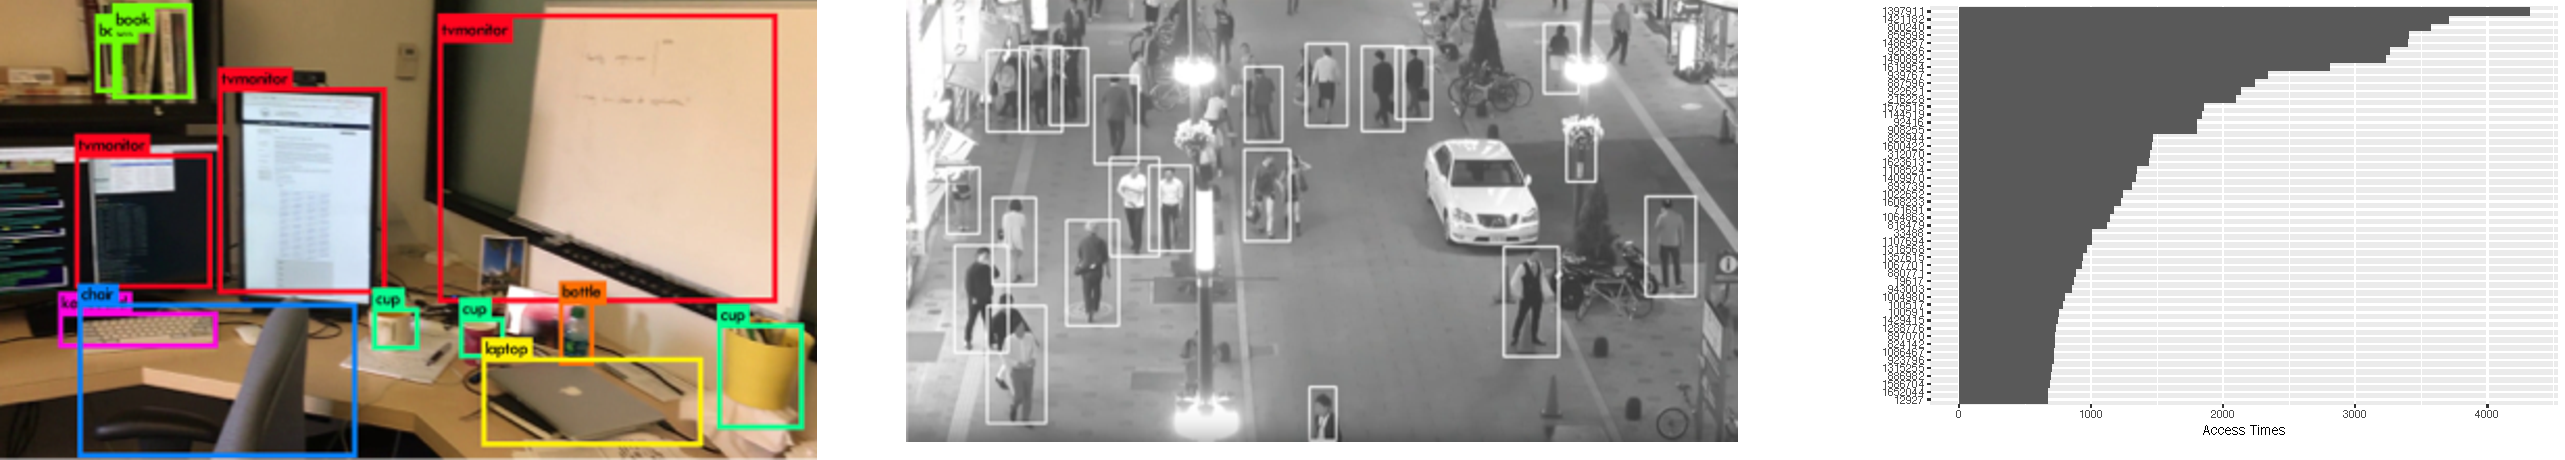
\includegraphics[width=\linewidth]{figures/apps.pdf}
\end{frame}

\begin{frame}{Top-K}
  \centering
  \begin{figure}
    \centering
    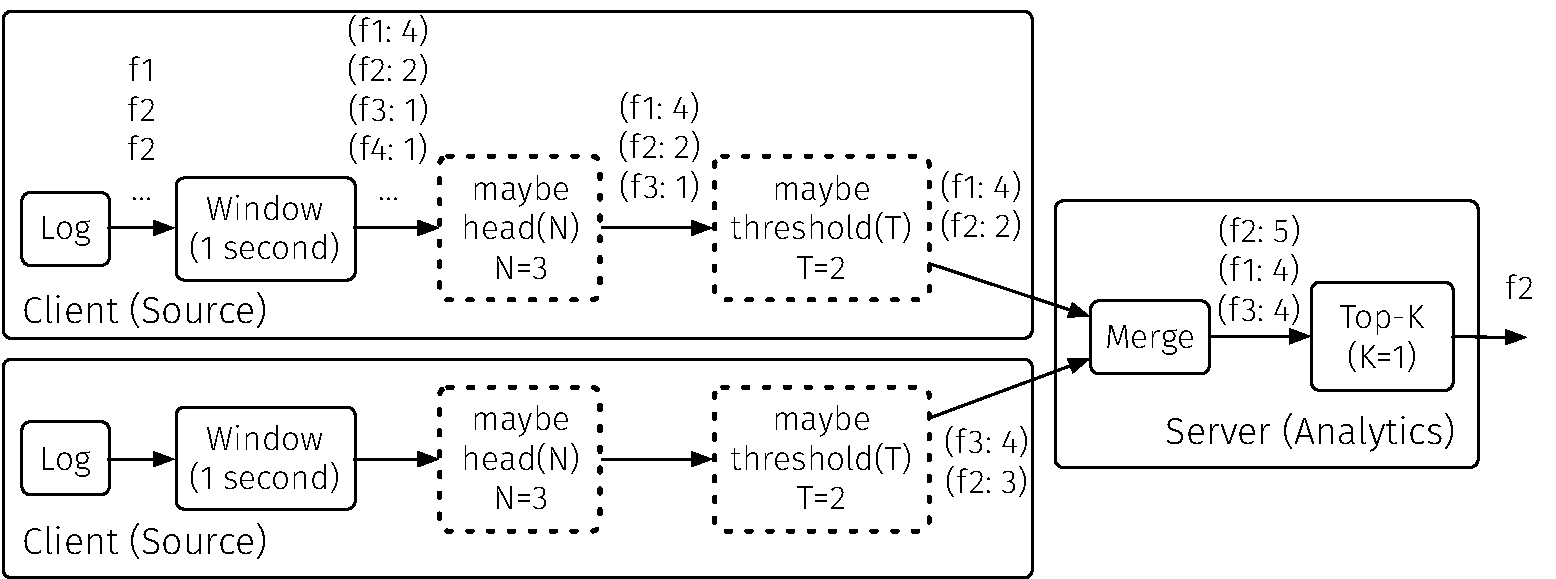
\includegraphics[width=\linewidth]{figures/topk.pdf}
    \caption{A distributed Top-K application with two degradation operations:
      \texttt{head} and \texttt{threshold}. In this example, \texttt{f2}, which
      is not in Top-1 for either client, becomes the global Top-1 after the
      merge. It would have been purged if the clients use threshold T=3,
      demonstrating degradation that reduces data sizes affects fidelity.}
    \label{fig:topk}
    \vspace{-0.5em}
  \end{figure}
\end{frame}

%%% Local Variables:
%%% mode: latex
%%% TeX-master: "../talk"
%%% TeX-engine: xetex
%%% End:
